%-----------------------------
% Packages
% ----------------------------

% -------------------
% Text Packages
% -------------------

\documentclass[final,5p,times,twocolumn]{elsarticle}


\usepackage{lineno}
\usepackage[hidelinks]{hyperref}

\usepackage[utf8]{inputenc}
\usepackage[T1]{fontenc}
\usepackage{tgbonum}
\usepackage{ragged2e}
\usepackage[svgnames,table,xcdraw]{xcolor}
\usepackage{lipsum}
\usepackage{lmodern}
\usepackage{listings}
\usepackage[version=4]{mhchem}
\usepackage{cuted}

% -------------------
% Figure Packages
% -------------------

\usepackage{graphicx} % Required for including pictures
\usepackage{subfigure}
\usepackage{wrapfig} % Allows in-line images
\usepackage[hypcap=false]{caption}
\usepackage{amsmath}
\usepackage[thinc]{esdiff}
\graphicspath{ {./images/} }
\usepackage{calc} % To reset the counter in the document after the title page
\usepackage{enumitem} % Includes lists
\newenvironment{Figure}
    {\par\medskip\noindent\minipage{\linewidth}}
    {\endminipage\par\medskip}
\usepackage{diagbox}

\usepackage{tikz}
\usepackage{tabularray}
\usepackage{array}

%-----------------------
% Set PDF Information
%-----------------------

\hypersetup{ 	
pdfsubject = {Year Abroad Level 11},
pdftitle = {Literature Review},
pdfauthor = {Daniel Markhoff}
}


% ---------------------
%
% Begin
%
% ---------------------



\def\pmbanner{{\hrule height 1 pt}\vskip35pt{Literature Review}\vskip35pt{\hrule height 4pt}\vskip20pt}

\begin{document}

\begin{frontmatter}



    \title{\pmbanner Particle Identification in Modern Cherenkov Detectors}
    
    \author{Danny Markhoff}
    \ead{d.markhoff@sms.ed.ac.uk, d.markhoff@gsi.de}

    %\affil[1]{\footnotesize School of Physics and Astronomy, University of Edinburgh, Mayfield Road, Edinburgh EH9 3FD, United Kingdom}
    %\affil[2]{\footnotesize GSI/FAIR, Planckstrasse 1, 64291 Darmstadt, Germany}

    \affiliation[1]{organization={University of Edinburgh}, 
                addressline={School of Physics and Astronomy, Mayfield Road},
                postcode={EH9 3FD}, 
                city={Edinburgh}, 
                country={United Kingdom}}

    \affiliation[2]{organization={GSI}, 
                addressline={Planckstrasse 1},
                postcode={64291}, 
                city={Darmstadt}, 
                country={Germany}}

\begin{abstract}
With major detector assemblies lining up for construction at high-energy facilities such as EIC and FAIR, 
technologies for particle identification are becoming ever more relevant. This review motivates the theory
of the field, introduces the technologies behind modern Cherenkov detectors, and discusses the implementation 
of these detectors into upcoming experiments.
Emphasis is placed on ......
Persistent challenges include ......
We conclude by outlining promising future developments for ......
\end{abstract}

\begin{keyword}
Particle Identification \sep Cherenkov Detectors \sep DIRC \sep RICH \sep PANDA \sep EIC \sep GSI
\end{keyword}

\end{frontmatter}

\begin{strip}
\vspace{-5em}
  \begin{flushright}
    \includegraphics[height=1.5cm]{Images/FAIR_Logo_cmyk.pdf}\hspace{1cm}%
    \includegraphics[height=1.5cm]{Images/UoE_Stacked Logo_CMYK_v1_160215.jpg}
  \end{flushright}

  \textit{For PwYA Literature Review} \hfill 6th January 2026

  \vspace{1em}

  Placement Supervisor: Dr. Jochen Schwiening \hfill j.schwiening@gsi.de

  Edinburgh Advisor: Dr. Moritz Pascal Reiter \hfill mreiter@ed.ac.uk

\end{strip}




\newpage
\twocolumn[{
  \begin{center}
    \vspace{1em}
    \tableofcontents
    \vspace{1em}
  \end{center}
}]

\clearpage
\section{Introduction}

\section{Theoretical Foundations}
\subsection{Cherenkov Radiation}
% filepath: /Users/danny/Documents/Courses/Year 4/Literature/Literature Review/PID-in-Modern-Cherenkov/Sections/Theoretical Foundations/cherenkov-radiation.tex
% Content for the "Cherenkov Radiation" subsection

\label{sec:cherenkov-radiation}

Cherenkov radiation is a phenomenon that occurs when a charged particle travels through a dielectric medium 
with refractive index \(n(\lambda)\) at a speed greater than the phase velocity in that medium. This effect 
was first observed by Pavel Čherenkov in 1934 \cite{Cherenkov_1937} and later explained theoretically by Ilya 
Frank and Igor Tamm \cite{Frank_1937}. 

\begin{figure}[h]
\centering
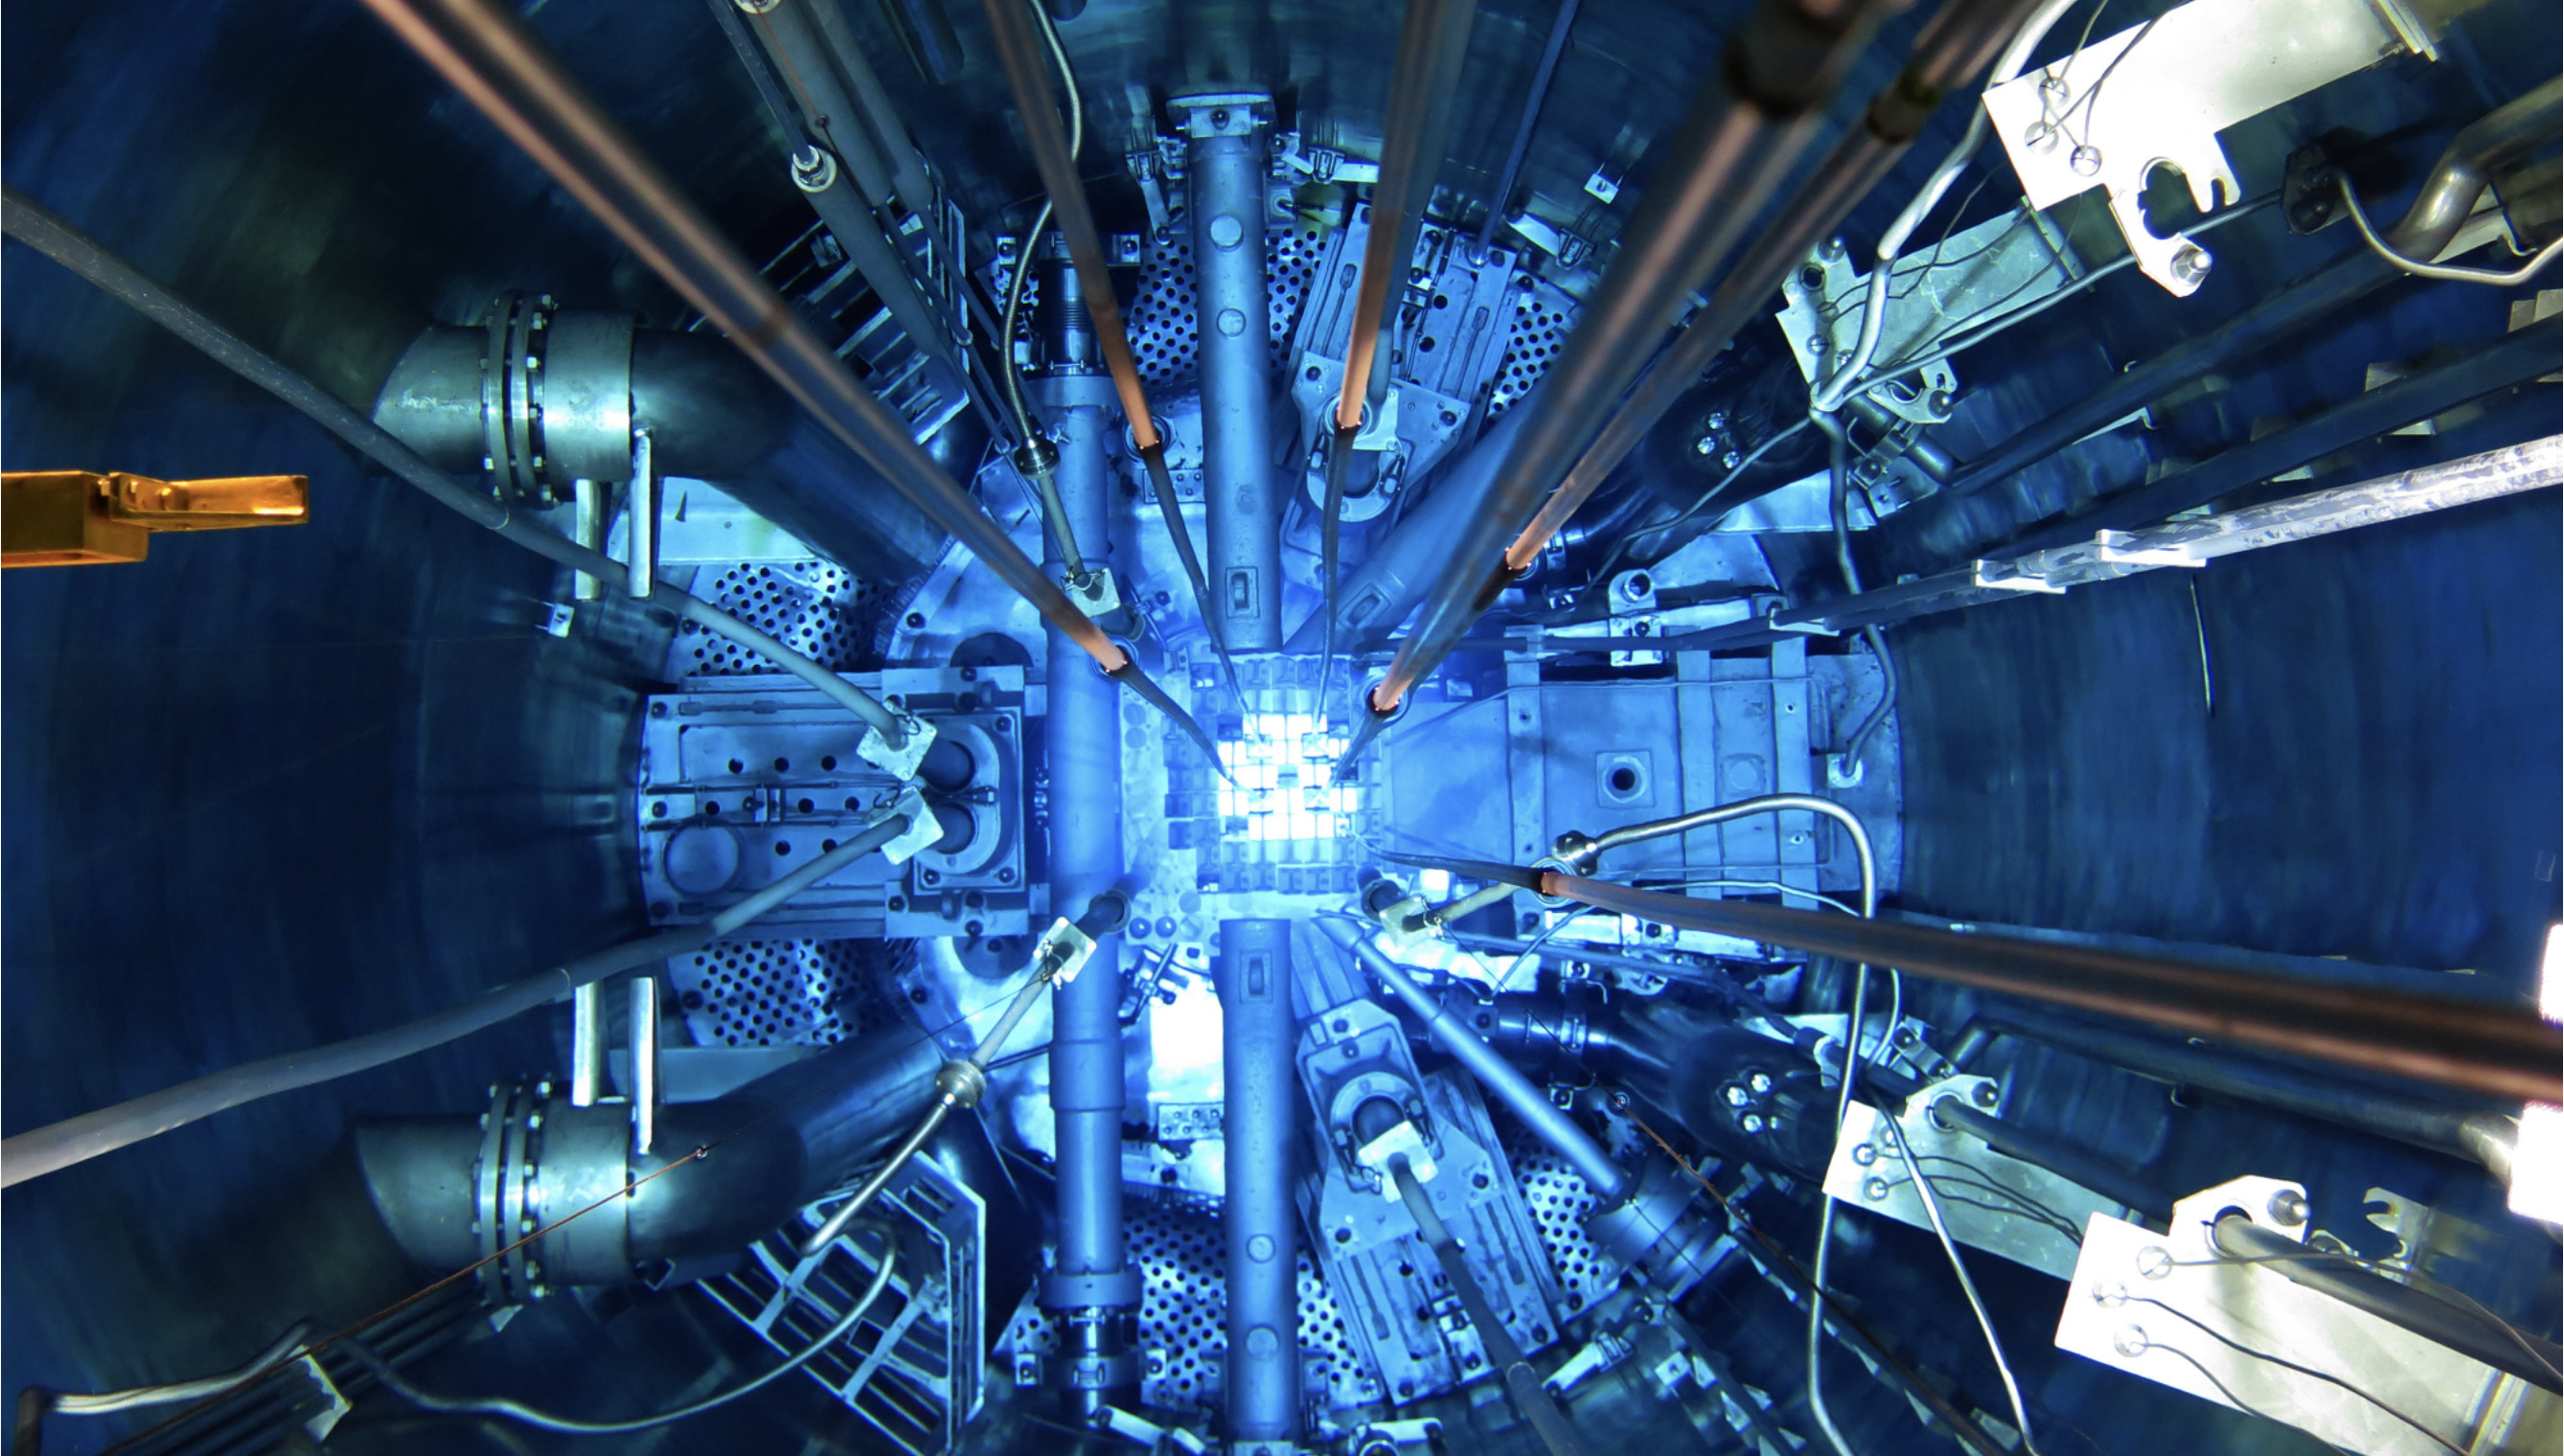
\includegraphics[width=\linewidth]{Images/cherenkov-light.png}
\caption{\textbf{Cherenkov radiation in a nuclear reactor pool.} The characteristic glow is indicative 
of relativistic electrons moving through the water. (Photo: IAEA)}\label{fig:cherenkov-light}
\end{figure}

From Maxwell's equations arises that electromagnetic propagation with wavelength \(\lambda\) will have its phase 
velocity modified by the medium it is travelling through. This leads to the idea of refractive index \(n(\lambda) = c/v\), 
defined as the ratio between the speed of light in vacuum \(c\) and the phase velocity \(v\) in the medium. The condition
for Cherenkov radiation to occur is then given by \(v > c/n\).

The Cherenkov radiation itself propagates at the phase velocity of the medium. As such, the radiation forms a 
conical wavefront with characteristic angle \(\theta\), similar to how shock cones are formed by supersonic 
aircraft. The angle \(\theta\) can be derived from simple geometric considerations shown in Fig \ref{fig:cherenkov-diagram}, yielding the following:

\begin{equation}
\cos{\theta} = \frac{v_p}{v} = \frac{c}{nv}
\label{equ:cherenkov-critical-angle}
\end{equation}

\begin{figure}[h]
\centering
\includegraphics[width=\linewidth]{Images/cherenkov-diagram.png}
\caption{\textbf{Schematic of a Cherenkov cone.} A particle travels through a medium with velocity \(v\). 
Photons are emitted at the phase velocity \(v_{p}\) and angle \(\theta\) to the path of travel of the particle, 
giving the characteristic blue shock cone.}\label{fig:cherenkov-diagram}
\end{figure}

The main principle behind a Cherenkov detector is to measure the angle \(\theta\) of the emitted photons,
which can then be used to determine the velocity \(v\) of the charged particle. With an associated momentum
measurement from a forward tracking detector, the mass of the particle can be inferred, allowing for spectroscopy.
This velocity spectroscopy for various particle species is shown in Fig \ref{fig:cherenkov-angle-COMPASS}.
It can be seen that pions, for example, will produce a larger Cherenkov angle than kaons or pions at the same momentum,
due to them being less massive.

\begin{figure}[h]
\centering
\includegraphics[width=\linewidth]{Images/cherenkov-angle.png}
\caption{\textbf{Cherenkov spectroscopy of the COMPASS RICH-1 detector at CERN.} There are clear curves for different 
particle species. These curves can be determined mathematically using \ref{equ:cherenkov-critical-angle} and relativistic
dynamics. (Photo: \cite{Tessarotto_2014})}\label{fig:cherenkov-angle-COMPASS}
\end{figure}

The energy \(dE\) emitted per unit length is given by the Frank-Tamm formula, which can be expressed as

\begin{equation}
\frac{dE}{dx} = \frac{q^2}{4\pi}\int_{v>\frac{c}{n(\omega)}}\mu(\omega)\omega\left( 1 - \frac{c^2}{v^2n^2(\omega)}\right) d\omega
\end{equation}

for a particle with charge \(q\) and frequency \(\omega\), moving through a medium with permeability \(\mu\) and 
refractive index \(n(\omega)\). The integral is taken over all frequencies where the Cherenkov condition \(v = c/n(\omega)\)
is met. By changing variables to wavelength \(\lambda\) and using that \(E = Nh\omega\), one can show that the 
number of photons \(N\) emitted per unit length is inversely proportional to the square of the wavelength. This
explains the characteristic blue of Cherenkov radiation, as shorter wavelength (blue light) photons are emitted more.




\subsection{Relativistic Kinematics}
\subsection{Optical Detector Theory}
\subsection{Particle Physics Motivation}
\subsection{Statistical Event Reconstruction Methods}
\subsection{Radiation-Matter Interactions}

\section{Photomultipliers}
\subsection{MCP-PMTs}
\subsection{SiPMs}
\subsection{LAPPDs}
\subsection{HRPPDs {\color{red} might get cut}}

\section{Photon Optics {\color{red} might get cut}}
\subsection{Lenses and Reflections}
\subsection{Laser Calibration}


\section{Ring Imaging Cherenkov Detectors (RICH)}
%Proximity Focusing RICH at ePIC
%ALICE at the LHC
%Belle II at SuperKEKB

\section{Detection of Internally Reflected Cherenkov Light (DIRC)}
%BaBar DIRC at SLAC
%hpDIRC at ePIC
%PANDA DIRC at FAIR

\section{Neutrino Identification with Cherenkov Detectors {\color{red} might get cut}}
\subsection{Atmospheric Muons}
\subsection{Water Cherenkov Detectors}
%IceCube Neutrino Observatory
%ANNIE FermiLab

\section{Applications at Future Facilities}
\subsection{PANDA DIRC at FAIR}
\subsection{hpDIRC at ePIC Brookhaven}
\subsection{Other Proposed Far Future Detectors {\color{red} might get cut}}

\section{Current Challenges and Limitations}
\subsection{ML PID}
\subsection{High Rate Environments}
\subsection{Radiation Damage}
\subsection{Budget Constraints}

\section{Emerging Technologies}
\subsection{HRPPDs}
\subsection{Advanced Optics}
\subsection{New Materials}

\section{Summary}

\cite{Singh_2019}


\bibliographystyle{ieeetr-modified} 
\bibliography{bibliography}

    \end{document}